\begin{question}
\noindent A UI/UX designer is sketching an icon on a grid before reflecting it to create a symmetrical logo.

\noindent Shape $S$ has vertices at $(3,1)$, $(3,4)$ and $(5,1)$.

\begin{center}
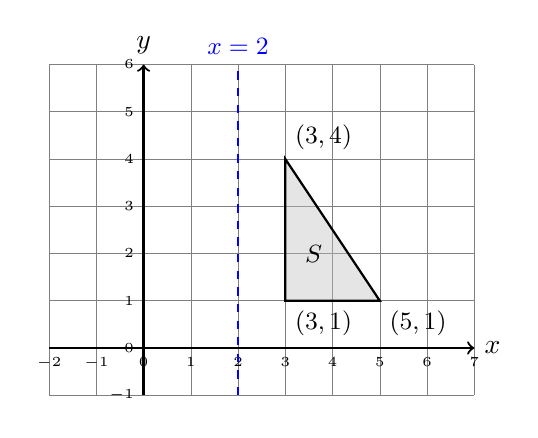
\begin{tikzpicture}[scale=0.6]
    % Grid
    \draw[step=1cm, gray, very thin] (-2,-1) grid (7,6);

    % Axes
    \draw[thick,->] (-2,0) -- (7,0) node[right] {$x$};
    \draw[thick,->] (0,-1) -- (0,6) node[above] {$y$};

    % Axis numbering
    \foreach \x in {-2,-1,0,1,2,3,4,5,6,7}
        \node[below, font=\tiny] at (\x,0) {$\x$};
    \foreach \y in {-1,0,1,2,3,4,5,6}
        \node[left, font=\tiny] at (0,\y) {$\y$};

    % Line of reflection x = 2
    \draw[dashed, thick, blue] (2,-1) -- (2,6);
    \node[above, font=\small, blue] at (2,6) {$x=2$};

    % Shape S
    \draw[thick, fill=lightgray, fill opacity=0.4] (3,1) -- (3,4) -- (5,1) -- cycle;
    \node[below right, font=\small] at (3,1) {$(3,1)$};
    \node[above right, font=\small] at (3,4) {$(3,4)$};
    \node[below right, font=\small] at (5,1) {$(5,1)$};
    \node[font=\small] at (3.6,2) {$S$};
\end{tikzpicture}
\end{center}

\noindent Reflect shape $S$ in the line $x = 2$.

\noindent On the grid, draw the image of shape $S$ after this reflection.

\vspace{5cm}

\begin{flushright}
\answerplain{2}
\end{flushright}
\end{question}
